\documentclass[pdf,fyma]{prosper}
%\usepackage[left=2cm,text={17cm, 24cm},top=3cm]{geometry}
\usepackage{times}
\usepackage[czech]{babel}
\usepackage[utf8]{inputenc}
\usepackage[T1]{fontenc}
\usepackage{graphics}
% ITY: Projekt 5, Andrej Barna (xbarna01), 2014/2015

\providecommand{\uv}[1]{„#1“}
\DefaultTransition{Replace}
\title{Typografie a publikování}
\subtitle{Projekt 5 - Vytváření prezentací}
\author{Andrej Barna}
\email{xbarna01@stud.fit.vutbr.cz}
\institution{Fakulta Informačních Technologií\\Vysoké Učení Technické v~Brně}
\slideCaption{PC Komponenty}

\begin{document}

\maketitle

\begin{slide}{Základná doska}
\begin{itemize}
\item ako názov napovedá, je základom počítača 
\item účelom je prepojiť komponenty počítača do funkčného celku
\item niektoré komponenty počítača sú v~nej zabudované, ako napríklad ROM alebo čipová sada
\item ostatné komponenty sa pripájajú buď do slotov, alebo pomocou káblov
\item vyrábajú sa v~rozličných veľkostiach pre odlišné využitia
\end{itemize}
\begin{figure}[ht]
  \begin{center}
  \scalebox{0.3}{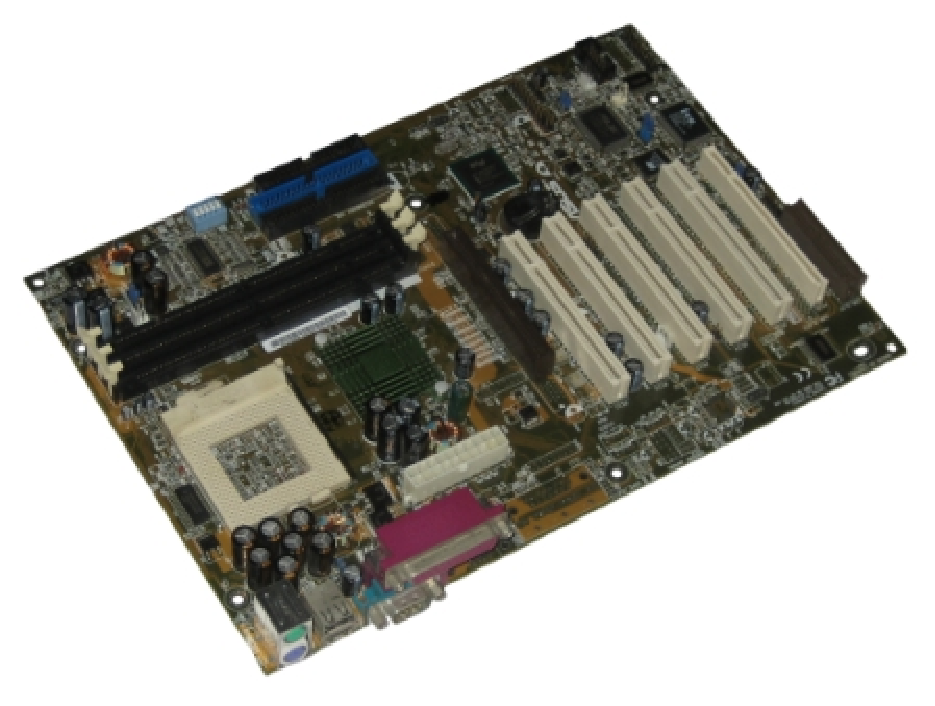
\includegraphics{motherboard.eps}}
  \label{motherboard}
  \end{center}
\end{figure}
\end{slide}

\begin{slide}{Procesor}
\begin{itemize}
\item \uv{mozog} počítača, vykonáva inštrukcie = beh programu
\item klasifikujú sa podľa viacerých kategórií -- šírka slova (veľkosť inštrukcie), počet jadier, \dots 
\item obsahuje niektoré iné komponenty, ako napríklad ALU, FPU či radič
\item má v~sebe zabudované registre a cache -- najrýchlejšie druhy pamäte
\end{itemize}
\begin{figure}[ht]
  \begin{center}
  \scalebox{0.5}{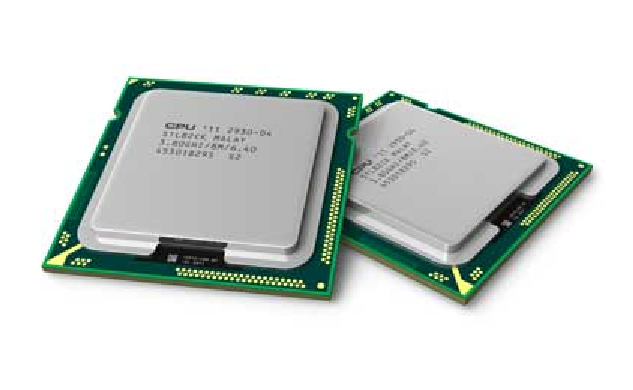
\includegraphics{cpu.eps}}
  \label{cpu}
  \end{center}
\end{figure}
\end{slide}

\begin{slide}{Pamäť RAM}
\begin{itemize}
\item RAM = Random Access Memory -- pamäť s~náhodným prístupom
\item pamäť s~rýchlym prístupom, ktorej obsah sa zmaže po odpojení z~napájania
\item prípaja sa priamo na základnú dosku do slotu pre ňu určeného
\item skladujú sa v~nej dáta operačného systému a bežiacich programov
\item existujú 2 druhy RAM: SRAM a DRAM
\begin{itemize}
\item SRAM pamäte sú drahé na výrobu a majú veľkú spotrebu energie, avšak sú rýchle a využívajú sa ako cache
\item DRAM pamäte sú lacné a majú nízku spotrebu, využívajú sa ako operačná pamäť, na ktorú referujeme bežne ako RAM
\end{itemize}
\end{itemize}
\end{slide}

\begin{slide}{Pevný disk}
\begin{itemize}
\item typ úložného zariadenia, ktorý je nevolatilný -- nestráca dáta po odpojení zdroja
\item je pomalší než pamäte RAM, avšak má väčšiu kapacitu
\item obsahuje rotujúce disky, z~ktorých číta dáta pomocou ramena, na konci ktorého je hlava čítača
\item bežne sa odlišujú na základe kapacity, veľkosti a počtu otáčok za minútu
\end{itemize}
\end{slide}

\begin{slide}{Disková mechanika}
\begin{itemize}
\item slúžia pre čítanie diskových pamäťových médií
\item bežné mechaniky podporujú viacero druhov diskov, najbežnejšie CD a DVD, či dokonca aj Blu-Ray disky
\item v~súčasnosti začínajú byť obľúbenejšie iné druhy prenosu dát, najmä veľkokapacitnými USB ukladacími zariadeniami
\end{itemize}
\begin{figure}[ht]
  \begin{center}
  \scalebox{0.5}{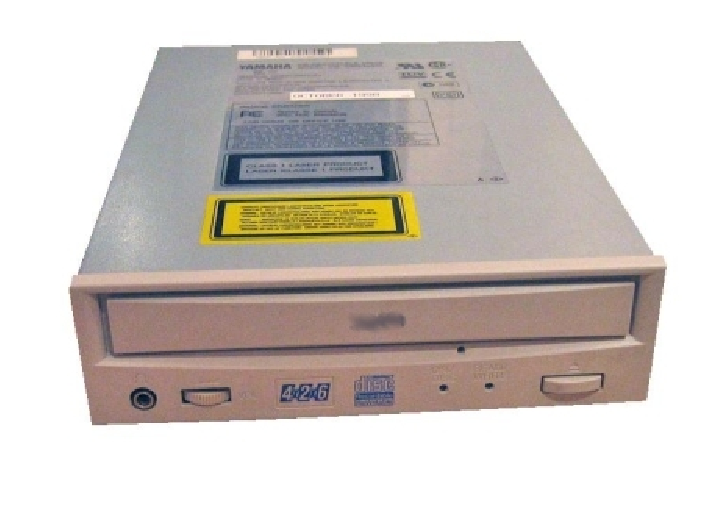
\includegraphics{cd_drive.eps}}
  \label{cd_drive}
  \end{center}
\end{figure}
\end{slide}

\begin{slide}{Zvuková karta}
\begin{itemize}
\item rozširujúca karta, ktorá spracováva vstupné a výstupné audio signály
\item zabudovaná na väčšine základných dosiek
\item ako všetky komponenty počítačov, aj zvukové karty prešli dlhým vývojom od schopnosti prehrávať jednoduché MIDI sekvencie, až po dnešné karty, schopné prehrávať multikanálové audio
\end{itemize}
\begin{figure}[ht]
  \begin{center}
  \scalebox{0.4}{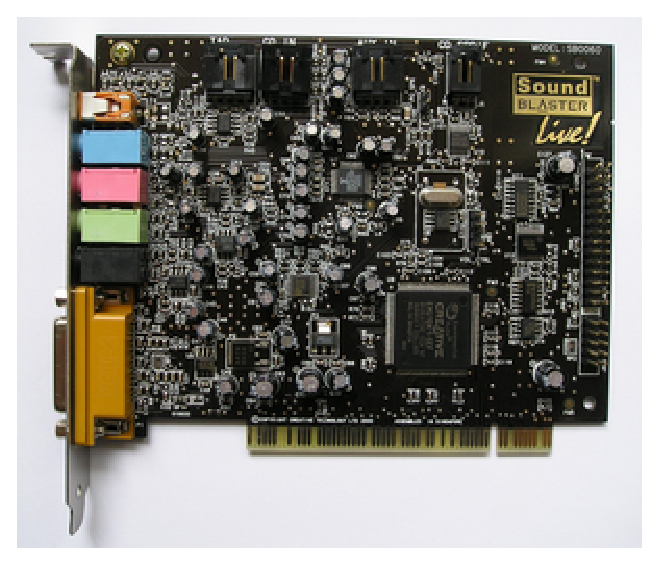
\includegraphics{sound.eps}}
  \label{sound}
  \end{center}
\end{figure}
\end{slide}

\begin{slide}{Grafická karta}
\begin{itemize}
\item príjma úlohy od CPU alebo APU, spracováva a tvorí grafický výstup na monitore
\item je bežne integrovaná do základnej dosky, avšak pre využitie pre 3D modelovanie či hranie hier nie je obvykle dostatočne výkonná
\item dokáže spracovávať aj pomocné výpočty pre CPU
\end{itemize}
\begin{figure}[ht]
  \begin{center}
  \scalebox{0.8}{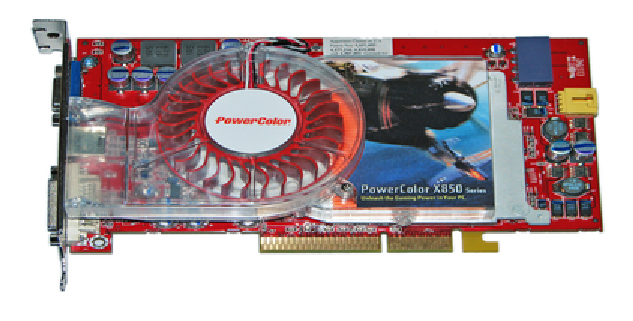
\includegraphics{graphics.eps}}
  \label{graphics}
  \end{center}
\end{figure}
\end{slide}

\begin{slide}{Sieťová karta}
\begin{itemize}
\item slúži ku vzájomnej komunikácii počítačov v~sieti
\item je často integrovaná na základnej doske, avšak v~minulosti bolo niekedy potrebné ju zapojiť
\item je to aktívne zariadenie -- vysiela a prijíma údaje
\item v~notebookoch sú často pre komunikáciu medzi zariadeniami alebo pripojenie sa na sieť často zabudované WiFi alebo Bluetooth adaptéry
\end{itemize}
\end{slide}

\begin{slide}{Zdroje}
\begin{itemize}
\item\tiny http://www.tutorialspoint.com/computer\_fundamentals/
\item\tiny http://openbookproject.net/courses/intro2ict/hardware/internal.html
\item\tiny http://cs.wikipedia.org/wiki/Grafick\%C3\%A1\_karta
\item\tiny http://cs.wikipedia.org/wiki/Zvukov\%C3\%A1\_karta
\item\tiny http://cs.wikipedia.org/wiki/S\%C3\%AD\%C5\%A5ov\%C3\%A1\_karta
\end{itemize}
\end{slide}

\end{document}